%! TEX program = lualatex
\documentclass[11pt]{scrartcl}
% Packages
\usepackage[margin=1.25in]{geometry}
\usepackage{index}
\usepackage{amsbsy} % Bold math symbols
\makeindex
\usepackage[utf8]{inputenc}
\usepackage[T1]{fontenc}
\usepackage{tcolorbox}
\tcbuselibrary{theorems}
\tcbuselibrary{skins}
\tcbuselibrary{breakable}
\usepackage{varwidth}
\usepackage{textcomp}
\usepackage{amsmath, amssymb}
\usepackage{esint}
\usepackage{titlesec}
\usepackage{xcolor}
\usepackage{titling}
\usepackage[linktocpage]{hyperref}
\usepackage{pgfplots}
\usepackage{multicol}
\setlength{\columnsep}{2em}
\usepackage{caption}
\usepackage{amsthm}
\usepackage{import}
\usepackage{cancel}
\usepackage{caption}
\usepackage{nicematrix}
\usepackage{mathrsfs}
\usepackage{mathtools}
%\usepackage{parskip}
\usepackage{pythonhighlight}
\usepackage{enumerate}
\usepackage{graphicx}
\usepackage[italian]{babel}
\usepackage{setspace}
\setstretch{1.2}
% To reset footnote numbering each page
\usepackage[perpage]{footmisc}
\usepackage{faktor}
\usepackage{tikz-cd}

% Titles 
\title{Appunti di\\ \vspace{.3cm} Algebra}
\author{Manuel Deodato}
\date{}


\definecolor{mastercolor}{HTML}{5666a8}


\newtheoremstyle{style1}% name of the style to be used
{5pt}% measure of space to leave above the theorem. E.g.: 3pt
{5pt}% measure of space to leave below the theorem. E.g.: 3pt
{\normalfont}% name of font to use in the body of the theorem
%{15pt}% measure of space to indent
{\parindent}% measure of space to indent
{\sffamily\scshape\bfseries}% name of head font
{}% punctuation between head and body
{ }% space after theorem head; " " = normal interword space
{\thmname{#1}\thmnumber{ #2}{\thmnote{ (#3)}.\ }}

\theoremstyle{style1}
\newtheorem{osservazione}{Osservazione}[section]
\newtheorem{teorema}{Teorema}[section]
\newtheorem{prop}{Proposizione}[section]
\newtheorem{corollario}{Corollario}[teorema]
\newtheorem{lemma}{Lemma}[teorema]
\newtheorem{definizione}{Definizione}[section]
\newtheorem{notazione}{Notazione}[section]
\newtheorem{esempio}{Esempio}[section]
\newtheorem{esercizio}{Esercizio}[section]

\newenvironment{svolgimento}{\renewcommand\qedsymbol{$\blacksquare$}\begin{proof}[Svolgimento]}{\end{proof}}

%% Generic box
\newtcolorbox{eqbox}[1][]
{
colback=gray!10,
arc=0pt,
boxrule=0pt,
title=#1
}

 \newenvironment{boxenv}[1][]{
    \begin{eqbox}[#1]
    }{
   \end{eqbox}
}



%%%%%%%%%% Medie con integrali multipli
\def\Yint#1{\mathchoice
    {\YYint\displaystyle\textstyle{#1}}%
    {\YYint\textstyle\scriptstyle{#1}}%
    {\YYint\scriptstyle\scriptscriptstyle{#1}}%
    {\YYint\scriptscriptstyle\scriptscriptstyle{#1}}%
      \!\iint}
\def\YYint#1#2#3{{\setbox0=\hbox{$#1{#2#3}{\iint}$}
    \vcenter{\hbox{$#2#3$}}\kern-.51\wd0}}
\def\longdash{{-}\mkern-3.5mu{-}} 
   % consider using "\mkern-7.5mu" if esint package is loaded
\def\tiltlongdash{\rotatebox[origin=c]{15}{$\longdash$}}
\def\fiint{\Yint\tiltlongdash}

\def\Zint#1{\mathchoice
    {\YYint\displaystyle\textstyle{#1}}%
    {\YYint\textstyle\scriptstyle{#1}}%
    {\YYint\scriptstyle\scriptscriptstyle{#1}}%
    {\YYint\scriptscriptstyle\scriptscriptstyle{#1}}%
      \!\iiint}
      \def\tilongdash{\mkern6mu{-}\mkern-4mu{-}\mkern-5mu{-}} 
   % consider using "\mkern-7.5mu" if esint package is loaded
\def\titiltlongdash{\rotatebox[origin=c]{15}{$\tilongdash$}}
\def\fiiint{\Zint\titiltlongdash}

%Captions
\captionsetup[figure]{font=footnotesize,labelfont=footnotesize}
\captionsetup[table]{font=footnotesize,labelfont=footnotesize}
%Titlesec
\titleformat{\section}
{\fontsize{18}{20}\sffamily\scshape}
{\normalfont\color{mastercolor}{\fontsize{18}{20}\selectfont\thesection}}
{0.7em}
{}
\titlespacing*{\section}{0pt}{*2}{1cm}
\titlespacing*{\subsection}{0pt}{*5}{.5cm}
\titlespacing*{\subsubsection}{0pt}{*5}{.5cm}

\hypersetup{colorlinks,breaklinks, linkcolor=[RGB]{86, 102, 168}}

% Personalizza la formattazione della subsection
\titleformat{\subsection}[block]{\centering\fontsize{14}{20}\bfseries}{\normalfont\thesubsection}{.5em}{}


% Personalizza la formattazione della subsubsection
\titleformat{\subsubsection}[block]{\centering\fontsize{12}{20}\bfseries}{\normalfont\thesubsubsection}{.5em}{}

% Maketitle customization
\renewcommand{\maketitle}{
\begin{center}
{\sffamily
{\fontsize{20}{20}\selectfont\MakeUppercase\thetitle}}

\vspace{0.2in}

{\large\scshape\sffamily\theauthor}
\end{center}
}

%Evaluate symbol
\DeclareMathOperator{\di}{d\!}
\newcommand*\Eval[3]{\left.#1\right\rvert_{#2}^{#3}}

%%%%%%% Numero delle equazioni in formato a.b
\numberwithin{equation}{subsection}
%%%%%

%%%%%%%%%% Personalizzazione numeri lista
\renewcommand{\theenumi}{(\arabic{enumi})}

%%%% Table of contents

\usepackage[titles]{tocloft}

\renewcommand{\cftdot}{}
\usepackage{titletoc}
%\setcounter{tocdepth}{2}

%%%%%%%%%%%%%%%% Toc style

% Personalizzazione scritta indice


% Font
%\usepackage{helvet}
%\renewcommand{\familydefault}{\sfdefault}	
%\renewcommand{\operatorname}[1]{\mathop{\mathrm{\textsf{#1}}}}
%\usepackage[noSTIXops,scaled=1.1]{newtxsf}
\renewcommand{\textbf}[1]{\textsf{\bfseries #1}}


\begin{document}
\maketitle
\vspace{9cm}
\begin{figure}[h!]
	\centering
	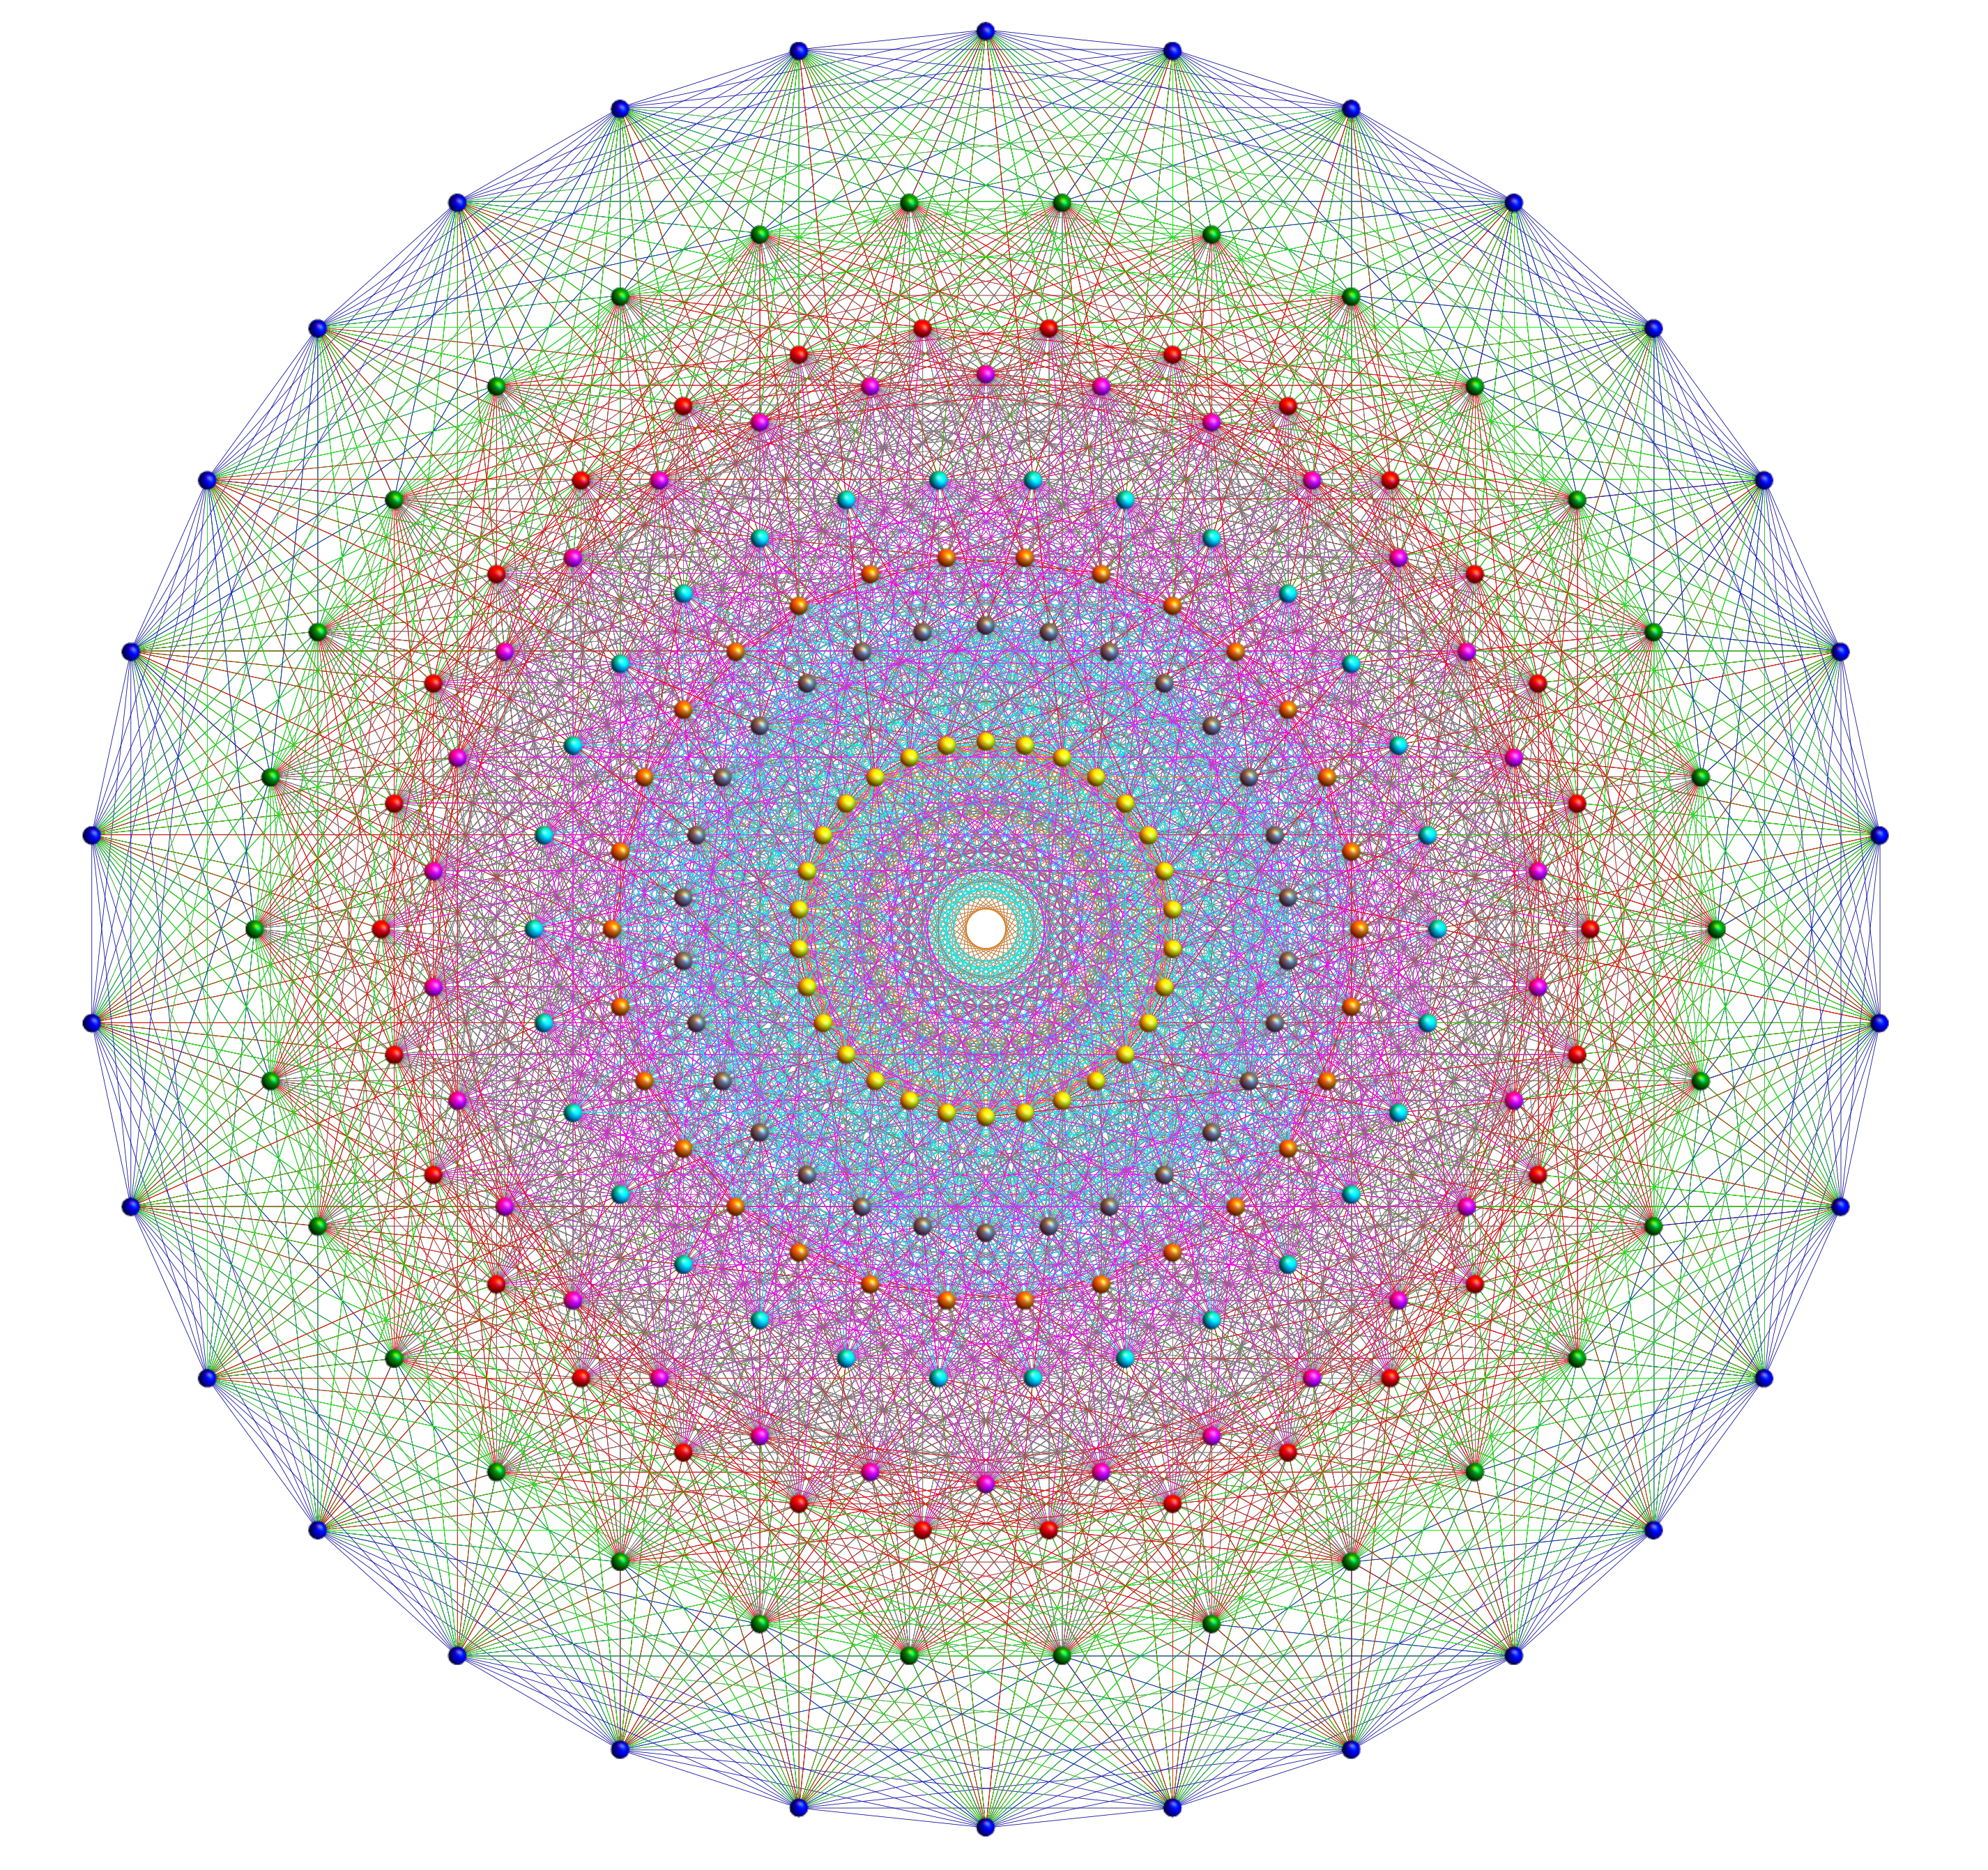
\includegraphics[width=.8\columnwidth]{front.jpeg}
\end{figure}

\newpage
\tableofcontents 
\newpage
\section{Teoria dei gruppi}
\subsection{Il gruppo degli automorfismi}
\begin{lemma}
	Siano $H,G$ due gruppi ciclici; un omomorfismo $\varphi : G \to H$ \`e univocamente determinato da come agisce su un generatore di $G$.
	\begin{proof}
		Sia $g_0\in G$ tale che $\langle g_0 \rangle = G$ e sia $\varphi (g_0) = \overline{h}\in H$.
		Per $g \in G$ generico, per cui $g_0^k = g$ per qualche intero $k$, si ha:
		\[
		\varphi (g) = \varphi (g_0^k) = \varphi (g_0)^k = \overline{h}^k
		\] 
		Cio\`e tutti gli elementi di $\operatorname{Im} \varphi $ sono esprimibili come potenze di $\overline{h}$.
	\end{proof}
\end{lemma}
\begin{osservazione}
Non ogni scelta di $\overline{h} \in H$ \`e ammissibile, ma bisogna rispettare l'ordine di $g_0$.
Se $g_0^n = e_G$, allora $e_H = \varphi (g_0^n) = \varphi (g_0)^n = \overline{h}^n$. Questa condizione, impone che $\operatorname{ord}(\overline{h})  \mid \operatorname{ord}(g_0) $.
\end{osservazione}
\begin{definizione}
	[Gruppo degli automorfismi]
	Sia $G$ un gruppo; si definisce il gruppo dei suoi automorfismi come
	\[
	\operatorname{Aut} (G) = \left\{ f: G \to G  \mid f \text{ \`e un isomorfismo di gruppi} \right\} 
	\] 
\end{definizione}
\begin{esempio}
	Si calcola $\operatorname{Aut} (\mathbb{Z})$. 
	\begin{svolgimento}
		Il gruppo $(\mathbb{Z},+)$ \`e ciclico, quindi un omomorfismo \`e determinato in base a come agisce su un generatore.
		Prendendo, per esempio $1$, si definisce $q_a :\mathbb{Z}\to \mathbb{Z} $ tale che $ q_a (1 ) = a$; perch\'e $\langle q_a(1) \rangle = \mathbb{Z}$\footnote{Richiesto dal fatto che $q_a$ sia suriettivo.}, \`e necessario che $a$ sia un generatore di $\mathbb{Z}$, perci\`o sono ammessi $a = \pm 1$. 
		In questo caso, $\operatorname{Aut} (\mathbb{Z})=\left\{ \pm \operatorname{Id} _{\mathbb{Z}}  \right\} \cong \left(\mathbb{Z} / 2\mathbb{Z}, +\right) $.
	\end{svolgimento}
\end{esempio}
\begin{teorema}
$\operatorname{Aut} (\mathbb{Z} / m \mathbb{Z}) \cong (\mathbb{Z} / m \mathbb{Z})^*$.
\begin{proof}
	$(\mathbb{Z} / m\mathbb{Z}, + )$ \`e ciclico, quindi si stabilisce l'azione di $f:\mathbb{Z} / m\mathbb{Z}\to \mathbb{Z}/ m\mathbb{Z}$ su un generatore.
	Preso, allora, $\overline{k} \in \mathbb{Z} / m\mathbb{Z} $ tale che $\operatorname{gcd}(k,m) =1$ e scelto $f(\overline{k}) = \overline{a}$, si ha che $\langle f(\overline{k}) \rangle= \langle \overline{a} \rangle= \mathbb{Z} / m\mathbb{Z} \iff \operatorname{gcd}(a,m) =1	\iff \overline{a} \in \left(\mathbb{Z} / m\mathbb{Z}\right) ^* $.
\end{proof}
\end{teorema}
\begin{definizione}
	[Automorfismo interno]
	Sia $G$ un gruppo; si definisce $\phi _g :G\to G$, $ \forall g \in G$, come $\phi_g (x) =gxg^{-1} $ ed \`e detto \textit{automorfismo interno}. 
	L'insieme di questi automorfismi, al variare di $g \in G$, forma il gruppo
	\[
	\operatorname{Int} (G) = \left\{ \phi _g : G\to G  \mid g \in G \text{ e } \phi _g \text{ automorfismo interno} \right\} 
	\] 
\end{definizione}
\begin{prop}\label{intcar}
	Sia $G$ un gruppo; allora $\operatorname{Int} (G) \lhd \operatorname{Aut} (G)$ e $\operatorname{Int} (G) \cong G / Z(G)$.
	\begin{proof}
		$\operatorname{Int} (G)$ \`e un sottogruppo di $\operatorname{Aut} (G)$ perch\'e $\operatorname{Id} (x) = exe^{-1} = x  \Rightarrow \operatorname{Id} \in \operatorname{Int} (G)$.
		Inoltre, $\phi _g \circ \phi _h (x) = ghxh^{-1}g^{-1}=\phi _{gh} (x) \in \operatorname{Int} (G)$ e $\phi _{g^{-1} } \circ \phi _g (x) = x \Rightarrow \phi _g^{-1} = \phi _{g^{-1}} \in \operatorname{Int}(G)  $.

		\`E un sottogruppo normale perch\'e $\forall f \in \operatorname{Aut} (G)$, si ha 
		\[
		f \circ \phi _g \circ f^{-1}(x) = f \left(g f^{-1}(x) g^{-1}\right) =f(g) x f(g)^{-1} \in \operatorname{Int} (G)
		\] 
		Per finire, si definisce $\Phi : G \to \operatorname{Int} (G) $.
		Questo \`e un omomorfismo perch\'e $\Phi(gh)=\phi _{gh} = \phi _g\circ \phi _h = \Phi(g)\Phi(h)$.
		\`E, inoltre, suriettivo perch\'e ogni automorfismo interno \`e associato ad un elemento di $G$, cio\`e $\forall \phi _g \in \operatorname{Int} (G), \ \exists g \in G : \Phi(g) = \phi _g$.
		Allora, la tesi deriva dal I teorema di omomorfismo, visto che $\operatorname{Ker} \Phi = Z(G)$.
	\end{proof}
\end{prop}
\begin{osservazione}\label{ossnorm}
	$H \lhd G \iff \phi _g(H) = H, \ \forall \phi _g \in \operatorname{Int} (G)$.
	\begin{proof}
Per ogni elemento di $\operatorname{Int} (G)$, si ha $\phi _g (H) = H \iff gH g^{-1} = H \iff H \lhd G$.
	\end{proof}
	\end{osservazione}
\begin{definizione}
	[Sottogruppo caratteristico]
	Sia $G$ un gruppo e $H < G$. Si dice che $H$ \`e \textit{caratteristico} se \`e invariante per automorfismo, cio\`e $\forall f \in \operatorname{Aut} (G), \ f(H) = H$.
\end{definizione}
\begin{corollario}
	Sia $G$ un gruppo; per la proposizione \ref{intcar} e l'osservazione \ref{ossnorm} se $H$ \`e caratteristico, allora $H \lhd G$.
\end{corollario}
\noindent Il viceversa \`e falso, cio\`e normale $\not\Rightarrow $ caratteristico; infatti, in $\mathbb{Z} / 2\mathbb{Z} \times  \mathbb{Z} / 2\mathbb{Z}$, il sottogruppo $\langle (1,0) \rangle$ \`e normale, ma non caratteristico perch\'e l'automorfismo che scambia le coordinate \`e tale per cui $\langle (1,0) \rangle\mapsto \langle (0,1) \rangle\neq \langle (1,0) \rangle$.
\subsection{Azioni di gruppo}
\begin{definizione}
	[Azione]
	Sia $G$ un gruppo; un'azione di $G$ su un insieme $X$ \`e un omomorfismo
	\[
	\gamma : 
	\begin{array}
		{c c c}
		G &\longrightarrow & S(X) = \left\{ f : X \to X  \mid f \text{ biettiva} \right\} \\
		g & \longmapsto & \psi _g : \psi_g(x) = g \cdot x
	\end{array}
	\] 
Pi\`u concretamente, si definisce \textit{azione} la mappa $\gamma : G \times  X\to X$ tale che
\begin{enumerate}[(a).]
	\item $e\cdot x = x$, per $e \in G$ e $x \in X$;
	\item $h\cdot (g\cdot x) = (hg)\cdot x$, per $g, h\in G$ e $x \in X$.
\end{enumerate}
\end{definizione}
\noindent Si verifica che una mappa $\gamma : G \times  X \to X$, con $G$ gruppo e $X$ insieme generico, che soddisfi le propriet\`a (a) e (b), \`e tale che $\gamma(g) (x) = \psi _g(x)$ (cio\`e a $g$ fissato) \`e biettiva.
\begin{proof}
	Per l'iniettivit\`a, si ha $\psi _g(x) = \psi _g(y) \iff g\cdot x = g\cdot y \iff x = y$, visto che si pu\`o applicare l'azione inversa $\gamma(g^{-1})$ ad entrambi i lati.
	Per la suriettivit\`a, invece, si nota che $\forall x \in X$, si trova anche una $y\in X: y= g^{-1}\cdot x$ dovuta all'azione di $\gamma(g^{-1})$, per cui $\psi _g(y)= g \cdot \left(g^{-1}\cdot x\right) =(gg^{-1}) \cdot x = x$.
\end{proof}
\begin{esempio}
Sia $G = \left\{ z \in \mathbb{C}^*  \mid  \lvert z \rvert =1 \right\} \cong S^1$ la circonferenza unitaria e $X = \mathbb{R}^2$.
Un'azione di $G$ su $X$ \`e una rotazione definita da $\gamma(z) = R(\operatorname{arg} z)$.
Questa \`e un omomorfismo perch\'e $\gamma(zw) = R(\operatorname{arg} zw)  = R(\operatorname{arg} z +  \operatorname{arg} w) = R(\operatorname{arg} z) R(\operatorname{arg} w)= \gamma(z) \gamma(w)$.
\end{esempio}
\noindent Un'azione $\gamma$ di $G$ su $X$ definisce, proprio su $X$, una relazione di equivalenza definita da 
\begin{equation}
	x \sim _\gamma y \iff x=\psi _g(y)=g \cdot y, \text{ con } x,y \in X
\end{equation}
La relazione di equivalenza \`e ben definita perch\'e le $\psi _g$ sono mappe biettive.
\begin{definizione}
	[Orbita]
	Sia $\gamma :G \to S(X)$ un'azione di $G$ gruppo su $X$. Dato $x \in X$, la sua classe di equivalenza rispetto alla relazione $\sim _\gamma$ \`e detta \textit{orbita} ed \`e indicata con $\operatorname{Orb} (x) = \left\{ g \cdot  x  \mid g \in G\right\} $.
\end{definizione}
\noindent Ricordando che una relazione di equivalenza fornisce una partizione dell'insieme su cui \`e definita, si ha:
\begin{equation}
	X = \bigsqcup_{x \in R} \operatorname{Orb} (x)
\end{equation}
con $R$ insieme dei rappresentati di tutte le orbite.
Se, poi, $X$ ha cardinalit\`a finita, allora:
\begin{boxenv}[]
\begin{equation}
	\lvert X \rvert  = \sum_{x \in R}^{} \lvert \operatorname{Orb} (x) \rvert 
\end{equation}
\end{boxenv}
\begin{definizione}
	[Stabilizzatore]
	Sia $\gamma: G \to S(X)$ un'azione di $G$ su $X$; allora per ogni $x \in X$, si definisce l'insieme 
	\[
	\operatorname{Stab} (x) = \left\{ g \in G  \mid g \cdot  x = x \right\} < G 
	\] 	
\end{definizione}
\begin{lemma}\label{l111}
	Sia $G$ un gruppo che agisce su un insieme $X$ e sia $x \in X$ un suo elemento. Dati anche $g\cdot x , h \cdot x \in \operatorname{Orb} (x)$ tali che $g \cdot x = h\cdot x$, allora $g$ e $h$ appartengono alla stessa classe di $G / \operatorname{Stab} (x)$.
\begin{proof}
	Se $g \cdot x, \ h\cdot x \in \operatorname{Orb} (x)$ sono uguali, allora $x =h^{-1} g \cdot x $, cio\`e $h^{-1} g \in G$ lascia invariato $x$, quindi \`e in $\operatorname{Stab} (x)$.
	Da questo segue che $h \operatorname{Stab} (x) = h h^{-1} g \operatorname{Stab} (x) = g \operatorname{Stab} (x)$.
\end{proof}
\end{lemma}
\begin{teorema}[Teorema di orbita-stabilizzatore]\label{osth}
	Esiste una mappa biettiva $\Gamma : \operatorname{Orb} (x) \to G / \operatorname{Stab} (x)$ tale che $\Gamma(g \cdot x) = g \operatorname{Stab} (x)$.
	\begin{proof}
		$\Gamma$ \`e iniettiva come diretta conseguenza del lemma \ref{l111} ed \`e suriettiva perch\'e $\forall g \operatorname{Stab} (x) \in G / \operatorname{Stab} (x), \exists g\cdot x \in \operatorname{Orb} (x)$ tale che $\Gamma(g\cdot x) = g \operatorname{Stab} (x)$.
		Segue che $\lvert \operatorname{Orb} (x)  \rvert = \lvert G \rvert / \lvert \operatorname{Stab} (x) \rvert $.
	\end{proof}
\end{teorema}
\begin{osservazione}
Si osserva che, per il teorema di orbita-stabilizzatore, la cardinalit\`a di un'orbita indica il numero di classi laterali dello stabilizzatore nel gruppo che compie l'azione, cio\`e il teorema di orbita-stabilizzatore si pu\`o riscrivere come $\lvert \operatorname{Orb} (x) \rvert = [G: \operatorname{Stab} (x)] = \lvert G / \operatorname{Stab} (x) \rvert = \lvert G \rvert / \lvert \operatorname{Stab} (x) \rvert $.
\end{osservazione}


\subsubsection{Azione di coniugio}
 Un caso notevole di azione \`e il coniugio: per $X=G$, si definisce $\gamma : G \to \operatorname{Int} (G) \subset S(G)$.
Le orbite indotte da questa azione sono dette \textit{classi di coniugio} e si indicano con $\operatorname{cl} (x)$, mentre lo stabilizzatore \`e detto \textit{centralizzatore} e si indica con:
\begin{equation}
	Z(x) = \left\{ g \in G  \mid g \cdot x = gxg^{-1} = x \right\} 
\end{equation}
Come conseguenza del teorema di orbita-stabilizzatore (\ref{osth}), si ha:
\begin{equation}
	\lvert G \rvert  = \lvert \operatorname{cl} (x)  \rvert  \lvert Z(x) \rvert , \ \forall x \in G
\end{equation}
\begin{prop}
	Sia $G$ un gruppo e $\gamma$ l'azione di coniugio su di esso; allora
	\[
	\bigcap_{x \in G} Z(x) = Z(G)
	\] 
	\begin{proof}
		Si ha $g \in Z(x), \ \forall x \iff gxg^{-1} =x , \ \forall x \in G \iff g \in Z(G)$.
	\end{proof}
\end{prop}
\begin{osservazione}
	[Centro di un sottogruppo]
	Sia $G$ un gruppo e $H < G$; allora il centro di $H$ \`e definito come 
	\[
	\bigcap_{x \in H}  Z(x) = Z(H)
	\] 
\end{osservazione}

\noindent Si considera, ora, l'azione di coniugio di un gruppo $G$ su $X = \left\{ H \subseteq G  \mid H< G \right\} $ e $\gamma(g) = \psi _g$ tale che $\psi_g (H) = gH g^{-1} $. 
Questa \`e un'azione ed \`e ben definita.
\begin{proof}
	Per dimostrare che \`e un'azione, si deve mostrare che la mappa $g \stackrel{\gamma}{\mapsto} \psi _g$ \`e un omomorfismo e che $\psi _g : X \to X$ sia biettiva.

	Si nota che $g \stackrel{\gamma}{\mapsto} \psi _g$ \`e un omomorfismo perch\'e $\psi _{g_1g_2} (H) = g_1g_2Hg_2^{-1}g_1^{-1} = \psi _{g_1} \circ \psi _{g_2} (H)$, cio\`e $g_1g_2\mapsto \psi _{g_1} \psi _{g_2} $.
	Inoltre, $\psi _g:X\to X$ \`e biettiva perch\'e $\exists \psi ^{-1} _g = \psi _{g^{-1}} : \psi _{g^{-1}} \circ \psi _g (H) = H $.

	Per mostrare che \`e ben definita, si fa vedere che effettivamente $\forall g, \psi_g$ mappa un sottogruppo di $G$ in un altro sottogruppo, cio\`e che $gHg^{-1} < G$.
	Intanto, $e \in gHg^{-1} $ perch\'e $H < G \Rightarrow  e \in H \Rightarrow geg^{-1}=e$; poi, $(ghg^{-1})(gh'g^{-1}) = ghh'g^{-1} \in g H g ^{-1}$ e $h^{-1} \in H \Rightarrow \exists (ghg^{-1} )^{-1} = g h^{-1}g^{-1}\in gHg^{-1}$ elemento inverso.
\end{proof}
\noindent Lo stabilizzatore di questa azione \`e detto \textit{normalizzatore}, in quanto \`e definito come tutti elementi di $G$ rispetto a cui $H$ \`e normale: 
\begin{equation}
	N_G(H) = \operatorname{Stab} (H) = \left\{ g \in G  \mid g H g^{-1}= H \right\} 
\end{equation}
Infine, l'orbita \`e l'insieme (classe di equivalenza) di tutti i coniugati di un sottogruppo di $G$:
\begin{equation}
\operatorname{Orb} (H) = \left\{ gHg^{-1}  \mid  g \in G \right\} 
\end{equation}
Per il teorema di orbita-stabilizzatore (\ref{osth}), si ha:
\begin{equation}
	\lvert G \rvert  = \lvert N_G(H) \rvert \lvert \operatorname{Orb} (H) \rvert 
\end{equation}
da cui si ricava anche che $H \lhd G \iff N_G(H) = G \iff \operatorname{Orb} (H) = \left\{ H \right\} $.
\subsubsection{Formula delle classi}

Si ricorda che le orbite definite da un'azione di un gruppo $G$ su un insieme $X$ formano una partizione di $X$ stesso, in quanto sono delle classi di equivalenza.
Se $\lvert X \rvert < \infty$, si ha:
\begin{equation}\label{ossclass}
\lvert X \rvert  = \sum_{x \in R}^{} \lvert \operatorname{Orb} (x) \rvert = \sum_{x \in R}^{} \frac{\lvert G \rvert }{\lvert \operatorname{Stab} (x) \rvert } = \sum_{x \in R'}^{} 1 + \sum_{x \in R \setminus R '}^{} \frac{\lvert G \rvert }{\lvert \operatorname{Stab} (x) \rvert }
\end{equation}
con $R$ insieme dei rappresentanti delle orbite e $R'$ insieme dei rappresentati delle orbite tali che $\operatorname{Orb} (x) = \left\{ x \right\} $, cio\`e degli elementi invarianti sotto l'azione di $G$. 
\begin{teorema}
	[Formula delle classi]
	Sia $\gamma:G \to S(G)$ l'azione di coniugio di un gruppo $G$ su un insieme $X$; allora:
	\begin{equation*}
		\lvert G \rvert  = Z(G) + \sum_{x \in R \setminus Z(G)}^{} \frac{\lvert G \rvert }{\lvert Z(x) \rvert }
	\end{equation*}
	\begin{proof}
		Segue per quanto appena detto e dall'osservazione che
		\[
		R' = \left\{ x \in R  \mid \operatorname{Orb} (x) = x \right\} = \left\{ x \in R  \mid gxg^{-1} = x \right\} = Z(G)
		\] 
		Visto che ogni orbita del genere contiene un solo elemento, i rappresentanti delle orbite sono esattamente tutti gli elementi di $Z(G)$, cio\`e un elemento $x \in Z(G)$ non pu\`o essere contenuto in nessun'altra orbita, se non nel singoletto $\left\{ x \right\} $.
		Perci\`o, la relazione in eq. \ref{ossclass}, avendo $X=G$, conferma la tesi.
	\end{proof}
\end{teorema}
\subsection{I p-gruppi}
\begin{definizione}
	[p-gruppo]
	Sia $p \in \mathbb{Z}$ un numero primo; allora si dice che $G$ \`e $p$-gruppo se $\lvert G \rvert = p^n$, per qualche $n \in \mathbb{N}$.
\end{definizione}
\begin{prop}\label{pnb}
	Il centro di un $p$-gruppo \`e non-banale.
	\begin{proof}
		Per la formula delle classi, si ha:
		\[
		p^n = \lvert Z(G) \rvert  + \sum_{x \in R \setminus Z(G)}^{} \frac{\lvert G \rvert }{\lvert Z(x) \rvert }
		\] 
		Se $\lvert Z(G) \rvert  = p^n$, la tesi \`e verificata, altrimenti $\exists x \in R \setminus Z(G)$, quindi tale che $Z(x) \subsetneq G$; allora, per qualche intero $k>0$, si ha $\lvert G \rvert / \lvert Z(x) \rvert = p^k$, da cui
		\[
		\lvert Z(G) \rvert =p^n - \sum_{x \in R \setminus Z(G)}^{} p^k\implies p  \mid \lvert Z(G) \rvert 
		\] 
		Visto che $e \in Z(G)$, deve risultare $\lvert Z(G) \rvert \ge 1$, da cui $\lvert Z(G) \rvert = p^s$, per qualche intero $s > 1$.
	\end{proof}
\end{prop} 
\begin{lemma}\label{GZGciffban}
	Vale $G / Z(G)$ ciclico $\iff G$ \`e abeliano.
	\begin{proof}
		Sia $G / Z(G)$ ciclico e sia $x_0 Z(G)$ il suo generatore.
		Date due classi laterali distinte $xZ(G), yZ(G) \in G / Z(G)$ e visto che $x_0Z(G)$ genera, si avr\`a $x_0^m Z(G)= x Z(G)$ e $x_0^nZ(G) = yZ(G)$, ossia, per $z,w \in Z(G)$, $x = x_0^m z,\ y = x_0^n w$. 
		Allora:
		\[
			 xy = x_0^m z x_0^n w = x_0^m x_0^n zw = x_0^n wx_0^m z = yx
		\] 
	Essendo questo valido per $x,y \in G$ generiche, si \`e dimostrata l'implicazione verso destra.

	Per l'implicazione inversa, sia $G$ abeliano; allora $Z(G) = G$ e $G / Z(G) = \left\{ e \right\} $, che \`e ovviamente ciclico.
	\end{proof}
\end{lemma}
\begin{prop}
	Un gruppo di ordine $p^2$ \`e abeliano.
	\begin{proof}
		Sia $G$ un $p$-gruppo tale che $\lvert G \rvert  = p^2$. Per mostrare che \`e abeliano, si fa vedere che $Z(G) = G$, ossia $\lvert Z(G) \rvert  = p^2$.
		Per la proposizione \ref{pnb}, si pu\`o avere solamente $\lvert Z(G) \rvert = p$, oppure $\lvert Z(G) \rvert = p ^2$.
		Se, per assurdo, fosse $\lvert Z(G) \rvert =p$, allora $\lvert G \rvert / \lvert Z(G) \rvert = p$, quindi $G / Z(G)$ avrebbe ordine primo e, quindi, sarebbe ciclico; per il lemma precedente (\ref{GZGciffban}), per\`o, questo \`e assurdo perch\'e risulterebbe anche abeliano al contempo, ma senza avere $\lvert Z(G) \rvert  = \lvert G \rvert $.
		Quindi deve essere $\lvert Z(G) \rvert  = p^2 = \lvert G \rvert \Rightarrow Z(G) = G$, da cui $G$ \`e abeliano.
	\end{proof}
\end{prop}
\subsection{Teoremi di Cauchy e Cayley}
\begin{lemma}[Teorema di Cauchy abeliano]\label{cab}
	Sia $p$ un primo e $G$ un gruppo abeliano finito; se $p  \mid  |G|$, allora $\exists x \in G : \operatorname{ord}(x) =p$.
	\begin{proof}
		Sia $\lvert G \rvert = pn$; si procede per induzione su $n$.
		Il passo base \`e ovvio: se $\lvert G \rvert =p$, allora \`e ciclico e, quindi, contiene un elemento di ordine $p$.

		Per il passo induttivo, si suppone che la tesi sia vera per ogni $m < n$ e si dimostra per $n$.

		Sia, allora $\lvert G \rvert  = pn$; sia, poi $y \in G, \ y\neq e$ tale che $\langle y \rangle= H < G$: per Lagrange, $\lvert G \rvert  = \lvert G / H \rvert  \lvert H \rvert $.
		Allora, se $p  \mid \lvert G \rvert \Rightarrow  p  \mid \lvert H \rvert $, oppure $ p   \mid \lvert G / H \rvert $.
		\begin{itemize}
			\item Se $p  \mid \lvert H \rvert $, allora pu\`o essere $\lvert G \rvert  = \lvert H \rvert $, caso in cui $G = \langle y \rangle$ sarebbe ciclico e, quindi, avrebbe un elemento di ordine $p$\footnote{In questo caso, l'elemento di ordine $p$ sarebbe proprio $y^{p^{n-1} } \in G $; infatti, $(y^{p^{n-1} } )^p = y^{p^n} = e$, visto che $|G| = p^n$.}, oppure pu\`o essere $\lvert H \rvert  = pm < pn$, caso in cui l'elemento di ordine $p$ \`e presente per ipotesi induttiva.
			\item Se $p  \mid  \lvert G / H \rvert $, invece, allora $\lvert G / H \rvert = pm' < pn$ perch\'e $H$ contiene almeno due elementi, cio\`e $y$ ed $e$; per ipotesi induttiva, allora, esiste $zH \in G / H$ il cui ordine \`e $p$.
				Considerando la proiezione $\pi_H : G \to G / H$ tale che $x \mapsto xH$ e ricordando che \`e un omomorfismo, si ha che, per questo motivo, $\operatorname{ord}(zH)  \mid \operatorname{ord}(z)\Rightarrow \operatorname{ord}(z) = pk$; se $k = n$, allora $G$ \`e ciclico e $z^n$ ha ordine $p$, altrimenti, se $k<n$, si ha la tesi per induzione.
		\end{itemize}
	\end{proof}
\end{lemma}
\begin{teorema}
	[Teorema di Cauchy]
	Sia $p$ un numero primo e $G$ un gruppo finito; se $p  \mid |G|$, allora esiste $x \in G : \operatorname{ord}(x) = p $.
	\begin{proof}
		Sia $|G| = pn$, con $p$ primo e $n \in \mathbb{N}$; si procede per induzione su $n$.
		Se $n=1$, $|G| = p \Rightarrow G$ \`e ciclico, quindi $\exists x \in G : \langle x \rangle=G$ e $\operatorname{ord}(x) = p$.

		Per il passo induttivo, si assume che la tesi sia valida per ogni $ m < n$ e si dimostra per $n$.

Si nota che se $\exists  H < G$ tale che $p  \mid  \lvert H \rvert $, allora $|H|=pm , \ m < n \Rightarrow \exists x \in H$ tale che $\operatorname{ord}(x) =p$ per ipotesi induttiva.
Si assume, dunque, che non esista alcun sottogruppo di $G$ il cui ordine sia divisibile per $p$.
Per la formula delle classi
\[
pn - \sum_{x \in R\setminus Z(G)}^{} \frac{\lvert G \rvert }{|Z(x)|} = \lvert Z(G) \rvert 
\] 
Ora, visto che $Z(x) < G \Rightarrow p$ non divide $|Z(x)|$, quindi si ha la certezza che, essendo $p  \mid |G| = |Z(x)| |G|/|Z(x)|$, $p$ divide $|G|/|Z(x)|$. 
Allora $p  \mid  |Z(G)|$, per cui $Z(G) =G$; infatti, se cos\`i non fosse, sarebbe un sottogruppo proprio di $G$ e $p$ non lo potrebbe dividere, il che \`e assurdo.

Da questo, segue che $G$ \`e abeliano, quindi la tesi segue dal teorema di Cauchy per gruppi abeliani (lemma \ref{cab}).
	\end{proof}
\end{teorema}
\begin{prop}\label{tgen}
Siano $H,K < G$; allora $HK < G \iff HK = KH$ e $\lvert HK \rvert = \lvert H \rvert \lvert K \rvert / \lvert H \cap K \rvert $.
\begin{proof}
Per la prima parte, \`e sufficiente osservare che per $hk \in HK$, l'elemento neutro $(hk)^{-1} = k^{-1} h^{-1} $ sta in $HK$ se e solo se $HK = KH$, e, allo stesso modo, il prodotto \`e chiuso cio\`e $hkh'k' = hh''k''k' \in HK$ solamente se $HK = KH$ cos\`i da poter trovare un elemento di $HK$ che sia uguale a $kh'\in KH$ che compare in tale prodotto.

La seconda parte, invece, si verifica considerando l'applicazione $\gamma: H \times K\to HK$ tale che $\gamma((h,k)) = hk$, che \`e evidentemente suriettiva; inoltre, se $s \in H \cap K$, allora $(hs,s^{-1}k) \in H \times K\Rightarrow \gamma ((hs,s^{-1}k)) = hk$, il che vuol dire che $\forall hk \in HK$, si trovano $|H\cap K|$ coppie in $H \times K$ che hanno immagine $hk$, da cui la tesi.
\end{proof}
\end{prop}
\begin{boxenv}[Classificazione dei gruppi di ordine 6]
Sia $G$ un gruppo di ordine $6$; per Cauchy, allora, esistono $x,y \in G$ tali che $\operatorname{ord}(x) = 2$ e $\operatorname{ord}(y) =3$. 
Se $G$ \`e abeliano, poi, si ha $\operatorname{ord}(xy) = 6$\footnote{Si dimostra per calcolo diretto; per esempio: $(xy)^3 = xyxyxy=xx x yyy=x$.}, quindi $G = \langle xy \rangle\cong \mathbb{Z}/ 6\mathbb{Z}$.

Se, invece, $G$ non \`e abeliano, si considera il sottogruppo $\langle x,y \rangle$ e si considera anche l'insieme $\langle x \rangle\langle y \rangle$ che, in generale, non \`e un sottogruppo.

Applicando la proposizione precedente (\ref{tgen}), si ha che $\lvert \langle x,y \rangle \rvert = (3 \cdot 2) / 1= 6$\footnote{L'intersezione \`e solo l'unit\`a perch\'e i due elementi hanno ordini diversi, quindi generano gruppi disgiunti.}, da cui $G = \langle x \rangle\langle y \rangle$, con $\langle x \rangle= \left\{ e,x \right\} $ e $\langle y \rangle= \left\{ e,y,y^2 \right\} $, quindi $G = \left\{ e , x ,y, xy,y^2 , xy^2 \right\} $.

Per finire, si mostra che $G \cong S_3$. 
Per farlo, si definisce $\phi :G \to S_3=\left\{ e,\tau ,\rho ,\tau \rho ,\tau ^2,\rho \tau ^2 \right\} $ tale che $\phi (x) = \rho $ e $\phi (y) = \tau $, con $\tau =(1,2,3)$ e $\rho = (1,2)$.
Questa mappa \`e suriettiva per costruzione, quindi \`e biettiva per questioni di cardinalit\`a; inoltre, \`e un omomorfismo, da cui segue la tesi.
\end{boxenv}

\begin{teorema}
	[Teorema di Cayley]
	Sia $G$ un gruppo; allora $G$ \`e isomorfo a un sottogruppo di $S(G)$.
	In particolare, se $|G| = n$, allora $G$ \`e isomorfo a un sottogruppo di $S_n$.
	\begin{proof}
		Si definisce l'azione
		\[
		\phi : 
		\begin{array}
			{c c c}
			G & \longrightarrow & S(G)\\
			g & \longmapsto & \gamma_g
		\end{array}, \ \text{ tale che } \gamma_g(x) = g\cdot x
		\] 
		Questa \`e ben definita perch\'e $\gamma:G \to G$ \`e biettiva, infatti $\gamma_g(x) = \gamma_g(y) \iff g \cdot x = g \cdot y \iff x = y$ e $\forall y \in G , \ \exists \gamma_g(g^{-1} \cdot y) = y $, il che mostra che \`e rispettivamente iniettiva e suriettiva.
		Inoltre, $\phi $ \`e un omomorfismo (ovvio) ed \`e anche iniettiva perch\'e $\operatorname{Ker} \phi = \left\{ g \in G  \mid \phi _g = \phi _e \right\} = \left\{ g \in G  \mid g \cdot x = x \right\} = \left\{ e \right\}$.
		Da questo, segue che $S(G)$ contiene una copia isomorfa a $G$.
	\end{proof}
\end{teorema}
\subsection{Commutatore e gruppo derivato}


\begin{definizione}
	Sia $G$ un gruppo e $S \subset G$ un suo sottoinsieme; allora $\langle S \rangle$ \`e il pi\`u piccolo sottogruppo di $G$ contenente anche $S$.
\end{definizione}
\begin{prop}
	Dato $G$ un gruppo e $S \subset G$ un suo sottoinsieme, vale la relazione
	\[
	\langle S \rangle= \left\{ s_1s_2 \ldots s_k  \mid k \in \mathbb{N}, \ s_i \in S \cup S^{-1} \right\} = X
	\] 
	con $S^{-1}= \left\{ s^{-1}  \mid  s \in S \right\} $.
	\begin{proof}
		Per definizione
		\[
			\langle S \rangle= \bigcap_{\substack{H < G \\ S \subset H}} H
		\] 
		Questa scrittura \`e ben definita perch\'e l'intersezione di gruppi \`e ancora un gruppo e, in questo modo, si ha il gruppo pi\`u piccolo contenente $S$; se cos\`i non fosse, ne esisterebbe uno pi\`u piccolo ancora, che, per\`o, farebbe parte dell'intersezione e sarebbe assurdo.

		Ora, per quanto detto sopra, $S$ \`e contenuto in tutti i gruppi la cui intersezione genera $\langle S \rangle$, quindi anche $S^{-1} $ deve essere contenuto in tali sottogruppi di $G$.
		Segue che $S,S^{-1}\subset H \Rightarrow X \subset H, \ \forall H < G$ e $S \subset H$, quindi $X \subset \bigcap H = \langle S \rangle$.

		Allo stesso tempo, $X$ \`e evidentemente un sottogruppo di $G$ e contiene $S$ per costruzione, quindi $X \supset \langle S \rangle$, da cui la tesi.
	\end{proof}
\end{prop}
\begin{definizione}
	[Commutatore]
	Sia $G$ un gruppo; dati $g,h \in G$, il loro \textit{commutatore} \`e definito come
	\[
		[g,h] = ghg^{-1} h^{-1}
	\] 
\end{definizione}
\begin{definizione}
	[Gruppo derivato]
	Dato un gruppo $G$, si definisce \textit{gruppo dei commutatori}, o \textit{derivato} di $G$, il gruppo 
	\[
		G ' = \langle [g,h]  \mid g,h \in G \rangle = [G:G]
	\] 
\end{definizione}
\noindent Ora si caratterizza il gruppo derivato.
Intanto, si ricorda che $\langle S \rangle$ \`e abeliano $\iff \forall s_1,s_2\in S , \  s_1s_2=s_2s_1$, $\langle S \rangle$ \`e normale $\iff \forall g \in G, \forall s \in S, \ gsg^{-1} \in \langle S \rangle$ e, infine, $\langle S \rangle$ \`e caratteristico $\iff \forall f \in \operatorname{Aut} (G) ,\ \forall s \in S$ si ha $f(s) \in S$.
Applicando queste alla definizione di commutatore, si ottiene la seguente.
\begin{prop}[Propriet\`a del derivato]\label{propderiv}
	
	Sia $G$ un gruppo e $G'$ il suo derivato; allora:
	\begin{enumerate}[(a).]
		\item $G ' = \left\{ e \right\}  \iff G$ \`e abeliano;
		\item $G' \lhd G$;
		\item $G'$ \`e caratteristico in $G$;
		\item dato $H \lhd G$, se $G / H$ \`e abeliano, allora $G' \subset H$.
	\end{enumerate}
	\begin{proof}
		La (a) \`e immediata perch\'e $G' = \left\{ e \right\} \iff \forall g_1,g_2 \in G, \ [g_1,g_2] = e $, cio\`e $g_1$ e $g_2$ commutano, da cui $G$ abeliano.

		Per la (b), $\forall x \in G, \ \forall g,h \in G $, si ha 
		\[
			\begin{split}
				x[g,h]x^{-1}  &= xghg^{-1}h^{-1}x^{-1}= xgx^{-1}xhx^{-1}xg^{-1}x^{-1}xh^{-1}x^{-1}\\
					      &=[xgx^{-1}, xhx^{-1}] \in G'
			\end{split}
		\] 
	Per la (c), si nota che $\forall f \in \operatorname{Aut} (G), \ \forall g,h \in G$, si ha:
	\[
		f([g,h]) = f(ghg^{-1}h^{-1}) = f(g) f(h) f(g)^{-1} f(h)^{-1} = [f(g), f(h)] \in G'
	\] 
	Infine, per la (d), se $H \lhd G$ e $G / H$ \`e abeliano, si ha $\forall x,y \in G$
	\[
		xHyH =yH xH\Rightarrow xyH = yxH \implies x^{-1}y^{-1}xy \in H \Rightarrow [x,y] \in H
	\] 
	da cui $H \supset G' $.
	\end{proof}
\end{prop}
\begin{corollario}
	Sia $G$ un gruppo e $G'$ il suo derivato; allora $G / G'$ \`e sempre abeliano ed \`e chiamato \textit{abelianizzazione} di $G$, nel senso che \`e il pi\`u grande quoziente abeliano di $G$.
	\begin{proof}
		Si mostra che $G / G'$ \`e sempre abeliano. 
		Siano, quindi $gG', hG' \in G / G'$ due classi laterali; allora si osserva che
		\[
			(gG') (hG') = ghG' = hg [g^{-1},h^{-1}] G' = hg G'
		\] 
		visto che $g^{-1}h^{-1}gh=[g^{-1},h^{-1}] \in G'$.
		Allora, dalla propriet\`a (d) della precedente proposizione (\ref{propderiv}), si ha $G' \subset H =G'$, cio\`e in questo caso si ha l'inclusione nell'insieme pi\`u piccolo, ovvero proprio $G'$. 
		Questo vuol dire che $G /G'$ \`e il quoziente con pi\`u elementi che sia abeliano perch\'e ottenuto tramite quoziente con $G'$, che \`e l'insieme pi\`u piccolo che soddisfa la propriet\`a\footnote{Per controposizione, se $G'\not\subset H\implies G/H$ non abeliano.}.
	\end{proof}
\end{corollario}
\subsection{Gruppi diedrali}
\begin{definizione}
	[Gruppo diedrale]
	Per $n \in \mathbb{N}$, si considera un $n$-agono regolare nel piano; l'insieme di tutte le isometrie del piano che mandano l'$n$-agono in se stesso \`e indicato con $D_n$ ed \`e noto col nome di \textit{gruppo diedrale}.
\end{definizione}
\begin{prop}
	Per $n \in \mathbb{N}$, il gruppo diedrale $D_n$ ha cardinalit\`a $\lvert D_n \rvert = 2n$.
	\begin{proof}
		Un'isometria \`e univocamente determinata dall'immagine di un vertice e di un lato adiacente al vertice stesso; allora, l'immagine pu\`o essere pari a $n$ possibili vertici, con due, conseguenti, possibilit\`a per il lato, da cui $2n$ possibili isometrie.
	\end{proof}
\end{prop}
\begin{prop}
	Sia $\rho $ una rotazione che sottende un lato\footnote{Cioè che manda un lato nel successivo.} e $\sigma $ una simmetria (riflessione) dell'$n$-agono regolare; allora $\rho ^n = e$, $\sigma ^2 =e$ e $\sigma \rho \sigma = \rho ^{-1} $.
	\begin{proof}
		Visto che $\rho $ manda un lato dell'$n$-agono regolare nella posizione del successivo, impiegher\`a $n$ iterazioni a far tornare il lato di partenza nella posizione originale; similmente, se $\sigma $ \`e una riflessione, sar\`a sufficiente riapplicarla per far tornare l'$n$-agono nella posizione originale.

		Per l'ultima, si nota che, componendo una rotazione e una riflessione, si ottiene una riflessione; applicando la seconda propriet\`a, si ottiene $\sigma \rho \sigma \rho = e \Rightarrow \sigma \rho \sigma  = \rho ^{-1} $.
	\end{proof}
\end{prop}
\begin{osservazione}
Le isometrie del piano che agiscono su un $n$-agono, quindi gli elementi di $D_n$, si possono mettere in relazione con $\mathrm{GL} _2(\mathbb{R})$, cio\`e possono essere rappresentate tramite matrici:
\begin{equation}
	\rho  \stackrel{\gamma}{\longmapsto} \begin{pmatrix} \displaystyle \cos \left(2\pi / n\right) & \sin \left(2\pi / n\right) \\ - \sin \left( 2\pi / n\right) & \cos (2\pi / n) \end{pmatrix}=M_\rho  \hspace{1cm}\sigma \stackrel{\gamma}{\longmapsto} \begin{pmatrix} 1 & 0 \\ 0 & - 1 \end{pmatrix} = M_\sigma 
\end{equation}
Si nota, inoltre, che indicando con $\mathbb{D}_n$ il gruppo generato da queste matrici, allora la mappa $\gamma : \langle \rho ,\sigma  \rangle\to \mathbb{D}_n$ e notare che questo \`e un omomorfismo di gruppi; infatti, la composizione di isometrie che fissano un punto, sono ancora isometrie che fissano lo stesso punto (in questo caso, l'$n$-agono).
Questo per dire che la mappa $\rho ^i \sigma ^j \mapsto M_\rho ^i M_\sigma ^j$ \`e ben definita.

Si pu\`o, inoltre, verificare che $M_\rho ^n = \operatorname{Id} $, $M_\sigma ^2 = \operatorname{Id} $ e $M_\sigma M_\rho M_\sigma = M_\rho ^{-1}$, per cui si conclude che $\gamma$ \`e un omomorfismo.

Essendo $\gamma$ un omomorfismo, si vede anche che $\rho $ e $\sigma $, come elementi di $D_n$, non sono legati da alcuna relazione perch\'e, altrimenti, lo sarebbero anche le loro matrici associate, cosa che sarebbe assurda. 
\end{osservazione}
\begin{prop}\label{dnitems}
	Tutti gli elementi di $D_n$ si scrivono come $\sigma \rho ^i$, oppure $\rho ^i$, con $i \in \left\{ 0,\ldots,n-1 \right\} $.
	\begin{proof}
	Sia $g \in D_n$; allora $g$ sar\`a una generica composizione di riflessioni e rotazioni del tipo $g= \rho ^{a_1} \sigma ^{b_1} \ldots \rho ^{a_k} \sigma ^{b_k} $, dove $a_i \in \mathbb{Z}$ e $b_j \in \left\{ 0,1 \right\} $. 
	Usando le relazioni $\sigma ^2 = \rho ^n = e$, si riscalano gli esponenti per scrivere $g = \rho ^{c_1} \sigma \ldots \rho ^{c_m} \sigma $, dove si sono anche, eventualmente, uniti esponenti di rotazioni consecutive (quindi $m\le k$).

	Usando $\sigma ^2 = e$ e assumendo $c_1\neq 0$, si pu\`o scrivere 
	\[
	g = \rho ^{c_1} \sigma \ldots \rho ^{c_m} \sigma = \sigma \sigma \rho ^{c_1} \sigma \sigma \sigma \rho ^{c_2} \ldots \sigma \rho ^{c_m} \sigma = \sigma \rho ^{-c_1} \rho ^{-c_2}  \ldots \rho ^{-c_m} = \sigma \rho ^{-d} 
	\] 
			dove si \`e fatto uso della relazione $\sigma \rho \sigma = \rho ^{-1} $ e con $d \equiv -\sum_{i=1}^{m} c_i \pmod{n} $.

			Se, invece, $c_1 = 0$ (cio\`e la \textit{parola} inizia con $\sigma $), allora $g = \rho ^{-c_2}\ldots \rho^{-c_m}  = \rho ^{d'}  $, con $d ' \equiv -\sum_{i=2}^{m} c_i \pmod{n} $.
			\end{proof}
\end{prop}
\noindent Grazie alla precedente proposizione, \`e possibile definire $\rho ^{[i]} = \rho ^i$, con $[i] \in \mathbb{Z} / n\mathbb{Z}$, visto che $\rho ^n = e$.

Inoltre, se $\rho ,\sigma  \in D_n$, allora $\langle \rho ,\sigma  \rangle< D_n$; per\`o, per quanto detto finora, si ha $\lvert \langle \rho ,\sigma  \rangle \rvert = 2n$ perch\'e $\rho ^n = e= \sigma ^2 $, quindi, per ragioni di cardinalit\`a, segue che $D_n = \langle \rho ,\sigma  \rangle$.

\subsubsection{Sottogruppi di $D_n$}
\hfill

\textbf{Numero di elementi di ordine k.} 
Sia $\rho $ una rotazione in $D_n$; si considera $\langle \rho  \rangle\cong C_n < D_n$\footnote{Qui, con $C_n$ si indica un generico gruppo ciclico di ordine $n$.}.

Essendo $C_n$ ciclico, vi sono $\phi (k)$ elementi di ordine $k$, se $k  \mid  n$.
Oltre alle $n$ rotazioni $\rho ^i$, in $D_n$ sono presenti anche le $n$ riflessioni $\sigma \rho ^i$; osservando che $\sigma \rho ^i \sigma \rho ^i = \rho ^{-i}\rho ^{i} = e $, si conclude che se $n$ \`e pari, vi sono $n+1$ elementi di ordine $2$ (cio\`e le $n$ riflessioni e $\rho ^{n / 2} $), mentre se $n$ \`e dispari, vi sono $n$ elementi di ordine $2$.
Ricapitolando:
\begin{equation}
\# \left\{ \text{elementi di ordine } k \right\} = \begin{cases}
	n + 1 &,\ \text{ se } k=2 \text{ e } n \text{ pari}\\
	n  &,\  \text{ se }k=2 \text{ e } n \text{ dispari}\\
	\phi (k)&,\ \text{ se } k \mid n\\
	0 &,\ \text{ altrimenti }
\end{cases}
\end{equation}
visto che le $n$ riflessioni sono tutte di ordine $2$ e l'esistenza di $\rho ^{n / 2} $ dipende dalla pairt\`a di $n$.
\vspace*{5pt}

 \textbf{I sottogruppi.} 
Nel punto precedente, si \`e notato che $C_n$ \`e uno dei sottogruppi.
Inoltre, i sottogruppi di $C_n$ sono noti: ne esiste uno per ogni divisore dell'ordine del gruppo, cio\`e $n$ in questo caso, per cui se $H < D_n$ e $H < C_n$, allora $H$ \`e l'unico sottogruppo di ordine $\lvert H \rvert $.
Se, invece $H< D_n$ e $H \not < C_n$, allora $H$ contiene almeno una riflessione $\tau $.
\begin{prop}
	Si ha $(H \cap C_n) \bigsqcup (\tau H \cap C_n) $ ed esiste una mappa biettiva tra $(H\cap C_n)$ e $(\tau H\cap C_n)$.
	\begin{proof}
		Si considera 
	\[
\begin{tikzcd}
D_n \arrow[r, "\gamma"] 
    \arrow[rr, bend right=30, "{\varphi }"'] & 
\mathrm{GL}_2(\mathbb{R}) \arrow[r, "\det"] & \{\pm 1\}\cong \mathbb{Z}/2\mathbb{Z}
\end{tikzcd}
\]
dove $\gamma$ \`e l'omomorfismo definito che a $\rho $ e $\sigma $ associa le relative matrici, mentre le matrici di $\mathrm{GL} _2(\mathbb{R})$ sono mappate a $\left\{ \pm 1 \right\} $ tramite il determinante: $\det M_\rho  = 1$ e $\det M_\sigma = -1$.
La mappa $\phi = \gamma\circ \det$ \`e un omomorfismo suriettivo proprio per come \`e definita $\gamma$ (cio\`e \`e un omomorfismo) e per il teorema di Binet per cui $\det (M^i_\rho M^j_\sigma ) = \det(M_\rho )^i \det (M_\sigma )^j = 1 ^i (-1)^j = 1 \iff j= 0$.

Considerando, quindi, $\varphi  :D_n \to \mathbb{Z} / 2\mathbb{Z}$, la sua restrizione $\varphi _H$ con $H < D_n$ e $H\not < C_n$ \`e suriettiva e il suo kernel \`e $H\cap C_n$; per il I teorema di omomorfismo, allora $H / (H\cap C_n) \cong \mathbb{Z} / 2\mathbb{Z}$.
Per il teorema di Lagrange, poi, si ha $\lvert H \rvert / \lvert H\cap C_n \rvert = \lvert \mathbb{Z} / 2 \mathbb{Z} \rvert $, per cui $\lvert H \rvert  = 2 \lvert H\cap C_n \rvert $.

Si nota che $\tau H \cap C_n \not \subset H \cap C_n$ perch\'e se $h \in H$, allora $\det (M_\tau M_h) = \det M_\tau \det M_h = -1$, per cui i due insiemi sono disgiunti; inoltre, $\tau h_1 = \tau h_2 \Rightarrow h_1=h_2$, per cui $\lvert \tau H \cap C_n \rvert = \lvert H \cap C_n \rvert $.
Considerando, allora
\[
\psi  : 
\begin{array}
	{c c c}
	H \cap C_n & \longrightarrow  & \tau  H \cap C_n\\
	h & \longmapsto &\tau  h
\end{array}
\] 
questa \`e biettiva.
Ora, $H \cap C_n = \langle \rho ^m \rangle= \left\{ e ,\rho ^m , \rho ^{2m} ,\ldots,\rho ^{n - m}  \right\} $, con $m  \mid  n$; se $\tau  = \sigma  \rho ^i $, allora 
\[
\tau  H \cap C_n = \left\{ \sigma \rho ^i, \sigma \rho ^{i+m}, \ldots, \sigma \rho ^{i+n - m}   \right\} 
\] 
quindi, l'unione dei due restituisce tutto $H$.
\end{proof}
\end{prop}
\noindent Segue che $H$ \`e composto da $m$ rotazioni e $m$ simmetrie; in particolare $H = \langle \rho ^m , \tau  \rangle\cong D_m$, quindi, se $m  \mid  n$, si hanno dei sottogruppi della forma $\mathbb{Z} / m \mathbb{Z}$ e $D_m$.
\vspace{5pt}

\textbf{Sottogruppi normali.} Per lo studio dei sottogruppi normali, si considerano le due seguenti proposizioni.
\begin{prop}
	Sia $G$ un gruppo e sia $H < G$; se $H$ ha indice $2$ in $G$, allora $H \lhd G$. 
	\begin{proof}
		Sia, quindi, $G / H = \left\{ H , \tau  H\right\} $, per qualche $\tau  \in G$; dato $g \in G$, allora, si ha $g = h_1$, oppure $g = \tau h_2$, con $h_1,h_2 \in H$. 
		Sia, ora, $hg \in Hg$ per $g \in G \setminus H$; allora $g = \tau  h_3$, oppure $hg = \tau h_4 = \tau h_3h_3^{-1}h_4= gh_5$, per cui $Hg \subset gH$. 
		Inoltre, $\lvert Hg \rvert =\lvert gH \rvert $, quindi deve essere $Hg = gH$ e, quindi, $H\lhd G$.
	\end{proof}
\end{prop}
\begin{prop}
	Siano $H \lhd G$ e $K < H$, con $K$ caratteristico in $H$; allora $K \lhd G$.
	\begin{proof}
		Si considera, per $g \in G$, $\phi _g : G\to G$ con $\phi_g(x) = gxg^{-1}$; per definizione, si ha $\phi _g (H) = H$, quindi $\phi_g|_{H} $ \`e un automorfismo, quindi $\phi _g|_{H} (K) = K, \ \forall g \in G \Rightarrow gKg^{-1} = K$, pertanto $K \lhd G$.
	\end{proof}
\end{prop} 

\noindent L'indice di $C_n$ in $D_n$ \`e $2$, quindi $C_n \lhd D_n$ per la prima proposizione.
Visto che per $G$ ciclico di ordine $n$, esiste un unico $H $, con $\lvert H \rvert =m  \mid n$, allora ogni sottogruppo di un gruppo ciclico \`e caratteristico e, quindi, nel caso di $D_n$, ogni sottogruppo di $\langle \rho  \rangle\cong C_n$ \`e caratteristico.
Per la seconda proposizione, questo significa che ogni sottogruppo di $C_n$ \`e normale; se $n$ \`e pari, allora $\langle \rho ^2  \rangle<C_n$ ha $n / 2$ elementi.

Considerando $H < D_n$ e $H \not \subset C_n$, con $H\cap C_n = \langle \rho ^2 \rangle$, si ha
\[
H=\langle \rho ^2 \rangle \sqcup \tau  \langle \rho ^2 \rangle
\] 
quindi $[D_n : H] = 2$, per cui $H \lhd D_n$.

Di sottogruppi di questa forma, se ne trovano due: $\langle \rho ^2 , \sigma  \rangle$ e $\langle \rho ^2 , \sigma \rho  \rangle$, ma non si sa se siano tutti i sottogruppi normali, quindi si cerca di caratterizzarli meglio.
Si sa che $H \lhd G \iff gHg^{-1}= H , \ \forall g \in G$, quindi per ogni elemento di un sottogruppo normale, devono figurare anche tutti i suoi coniugati.
Per la proposizione \ref{dnitems}, per capire come sono fatti i coniugati di $D_n$, \`e sufficiente studiare quali siano quelli di $\rho ^i$ e $\sigma \rho ^i$. 
Si nota che:
\[
\rho ^i \rho ^i \rho ^{-i}= \rho ^i \hspace{1cm}\sigma \rho ^i \rho ^i \rho ^{-i}\sigma  = \sigma \rho ^i\sigma =\rho ^{-i}
\] 
quindi l'insieme dei coniugati di $\rho ^i$ \`e $\left\{ \rho ^i, \rho ^{-i} \right\} $; in particolare, se $i \in \left\{ 0 , n /2 \right\} $, tale insieme diventa $\left\{ e \right\} $, oppure $\left\{ \rho ^{ n / 2}  \right\} $ rispettivamente.
Poi, si nota che:
\[
\rho ^i \sigma \rho ^j \rho ^{-i}= \sigma \rho ^{-i}\rho ^j\rho ^{-i}=\sigma \rho ^{j-2i} \hspace{1cm} \sigma \rho ^i\sigma \rho ^j \rho ^{-i} \sigma = \rho ^{-i}\rho ^j\rho ^{-i}\sigma =\sigma \rho ^{2i-j} 
\] 
quindi se $n$ \`e pari, allora $\sigma \rho ^s \sim \sigma \rho ^t\iff  \equiv t \pmod{2} $, quindi le riflessioni di spezzano in due classi di coniugio; se $n$ \`e dispari, invece, le riflessioni sono tutte coniugate.

Ricapitolando: 
\begin{itemize}
	\item se $n$ \`e dispari e se un sottogruppo contiene una riflessione, allora le contiene tutte e tutte le riflessioni generano $D_n$, infatti $\sigma $ \`e dato e $\rho  = \sigma \sigma \rho $, quindi $H \lhd D_n \Rightarrow H = D_n$, mentre se non contiene alcuna riflessione, allora \`e un sottogruppo di $C_n$;
	\item se $n$ \`e pari, oltre ai sottogruppi di $C_n$, si considerano gli $H\lhd D_n$ che sono tali che $\sigma \rho ^i \in H$, per cui $\sigma \rho ^{i+2} \in H$ e $\rho ^2 \in H$, pertanto, se $H \neq D_n$, devono essere della forma $\langle \rho ^2,\sigma  \rangle$, o $\langle \rho ^2,\sigma \rho  \rangle$.
\end{itemize}

\textbf{Sottogruppi caratteristici.}
Usando quanto visto per i sottogruppi normali, si conclude che i possibili sottogruppi caratteristici sono i sottogruppi di $C_n$ e $\langle \rho ^2,\sigma  \rangle$ e $\langle \rho ^2 , \sigma \rho  \rangle$. 
Mentre si sa gi\`a che i sottogruppi di $C_n$ sono caratteristici, si osserva che, per gli altri due, la mappa $\tau : D_n \to D_n$ tale che $\tau (\rho ) = \rho $ e $\tau (\sigma ) = \sigma \rho $ ]`e un automorfismo che scambia $\langle \rho ^2,\sigma  \rangle$ con $\langle \rho ^2, \sigma \rho  \rangle$ e viceversa, quindi non sono caratteristici.
\subsubsection{Centro, quozienti e automorfismi di $D_n$}
\hfill

\textbf{Il centro.} Si cercano tutti gli elementi $\tau  \in D_n$ tale che $\forall \rho  \in D_n, \ \rho \tau \rho ^{-1}=\tau $.
Dal precedente studio dei coniugi nei sottogruppi normali, si conclude che $Z(D_n) = \left\{ e \right\} $ se $n$ \`e dispari e $Z(D_n)=\left\{ e, \rho ^{n / 2}  \right\}\cong \mathbb{Z} / 2\mathbb{Z}$ se $n$ \`e pari.

\vspace{5pt}

\textbf{Quozienti.} 
Si sa che i quozienti sono in corrispondenza biunivoca con i sottogruppi normali, il che vuol dire che esiste un quoziente per ciascun $H \lhd G$.
A meno di un automorfismo, i quozienti si ottengono come segue.
Per quanto visto precedentemente, i sottogruppi normali sono i sottogruppi di $C_n$ e, se $n$ \`e pari, anche quelli della forma $\langle \rho ^2 , \sigma  \rangle$ e $\langle \rho ^2, \sigma \rho  \rangle$. 
Sia, $\langle \rho ^m \rangle< C_n$, con $ m \mid n$, per cui $\lvert D_n / \langle \rho ^m \rangle \rvert = 2n/m$.
\begin{prop}
	Si ha $D_n / \langle \rho ^m \rangle\cong D _{n / m} $.
	\begin{proof}
		Si considera 
		\[
		\gamma : 
		\begin{array}
			{c c c}
			D_n & \longrightarrow& D_{ n / m } \\
			\sigma &\longmapsto & \tau \\
			\rho  &\longmapsto & \epsilon 
		\end{array}
		\] 
		dove $D_n = \langle \sigma ,\rho  \mid \rho ^n = \sigma ^2 = e , \sigma \rho \sigma = \rho ^{-1} \rangle$ e $D_{n / m} = \langle \tau ,\epsilon  \mid \epsilon ^{ n / m} = \tau ^2 = e , \ \tau \epsilon \tau \epsilon ^{-1} \rangle$.
		Si nota che questo \`e suriettivo e il suo nucleo \`e $\langle \rho ^m \rangle$, quindi si ha la tesi per il I teorema di omomorfismo.
	\end{proof}
\end{prop}
\noindent Nel caso di $n$ pari, poi, vi sono gli altri due sottogruppi citati sopra, che hanno indice $2$ e, quindi, i cui quozienti sono isomorfi a $\mathbb{Z} / 2\mathbb{Z}$.

\vspace{5pt}
\textbf{Gli automorfismi.} 
Si studia $\operatorname{Aut} (D_n)$. Per farlo, si cerca di calcolarne la cardinalit\`a.
Per definire un automorfismo in $D_n$, lo si definisce sui generatori, che si sanno essere $\rho $ e $\sigma $.
L'immagine di questi generatori deve essere un altro generatore: ad esempio, l'immagine di $\rho $, che ha ordine $n$, deve avere come immagine un elemento di ordine $n$; questi sono della forma $\rho ^i$, con $\operatorname{gcd}(i,n) =1$, quindi ci sono $\phi (n)$ possibili scelte.
Poi, $\sigma $ ha ordine $2$ e deve avere, come immagine, un altro elemento di ordine $2$ che, insieme al $\rho ^i$ scelto prima, generi $D_n$; ci sono $n$ riflessioni della forma $\sigma \rho ^j$, quindi un totale di $n$ scelte possibili.
Si nota che se $n$ \`e pari, anche $\rho ^{ n / 2} $ ha ordine $2$, ma la coppia $\rho ^i, \rho ^{n / 2} $ non genera $D_n$.

Sia, allora 
\[
\gamma : 
\begin{array}
	{c c c}
	D_n & \longrightarrow & D_n\\
	\rho ^h & \longmapsto & \rho ^{ih} \\
	\sigma \rho ^k & \longmapsto & \sigma \rho ^j \rho ^{ik} 
\end{array}
\] 
con $\operatorname{gcd}(i,n) =1$ e $j$ qualsiasi; $\gamma$ \`e ben definita e 
\[
\gamma\left((\rho ^s)(\sigma \rho ^t)\right) = \gamma(\sigma \rho ^{t-s} )= \sigma \rho ^j \rho ^{i(t-s)} = \sigma \rho ^{-is} \rho ^j \rho ^{it} = \rho ^{is} \sigma \rho ^j\rho ^{it} = \gamma(\rho ^s)\gamma(\sigma \rho ^t)
\] 
per cui \`e un omomorfismo. 
Inoltre, \`e biettiva per costruzione, quindi si ha $\lvert \operatorname{Aut} (D_n) \rvert = n \phi (n)$; da un punto di vista insiemistico, esiste una biezione tra $\operatorname{Aut} (D_n)$ e $\mathbb{Z} / n\mathbb{Z} \times \left(\mathbb{Z} / n\mathbb{Z}\right) ^*$.
\begin{esercizio}
	Studiare $D_4$ (risultati a pagina 19) e $D_6$.
\end{esercizio}
\subsection{Permutazioni}
\begin{definizione}
	[Permutazione]	
	Sia $X$ un insieme; una mappa $f : X \to X$ \`e detta \textit{permutazione} se \`e biettiva. 
	Le permutazioni formano un gruppo rispetto alla composizione tra funzioni ed \`e indicato con
	\[
	S(X) = \left\{ f : X \to X  \mid  f \text{ \`e biettiva} \right\} 
	\] 
	Se $X = \left\{ 1,\ldots, n \right\} $, allora il gruppo delle permutazioni si indica con $S_n$ e $\lvert S_n \rvert  = n!$.
\end{definizione}
\noindent Una permutazione di $S_n$ pu\`o essere rappresentata tramite cicli, i quali sono disgiunti e, quindi, commutano fra loro.

Ogni $k$-ciclo (ciclo di lunghezza $k$) ha $k$ scritture diverse, tutte equivalenti fra loro, dovute alla possibilit\`a di scegliere uno fra i $k$ elementi del ciclo come primo elemento; dopo questa scelta, tutti gli altri sono univocamente determinati.
\begin{prop}
	I cicli di una permutazione di $S_n$ sono orbite degli elementi di $X = \left\{ 1,\ldots,n \right\} $ formate dall'azione indotta da tale permutazione.
	\begin{proof}
		Sia $\sigma \in S_n$ e sia $\langle \sigma  \rangle$ il sottogruppo ciclico generato da $\sigma $.
		Si considera l'azione di $\langle \sigma  \rangle$ su $X$ secondo la legge $\sigma ^k \cdot x = \sigma ^k (x)$; l'orbita di ciascun elemento di $X$ \`e della forma
		\[
		\operatorname{Orb} (x) = \left\{ \sigma ^k(x)  \mid  k \in \mathbb{Z} \right\} 
		\] 
		Si nota che $\lvert X \rvert < \infty \Rightarrow  \lvert \operatorname{Orb} (x) \rvert < \infty, \ \forall x$. 
		Sia, poi, $m\ge 1$ il pi\`u piccolo intero tale che $\sigma ^m(x) = x$\footnote{Questo esiste per forza, altrimenti si avrebbero orbite di infiniti elementi a partire da un insieme finito.}; allora gli elementi 
		\[
		x, \ \sigma (x) , \ \sigma ^2 (x) , \ldots,\ \sigma ^{m-1} (x)
		\] 
		sono tutti distinti (per definizione di $m$) e formano $\operatorname{Orb} (x)$.
		Facendo agire $\sigma $ su $\operatorname{Orb} (x) \subset X$, si nota che 
		\[
		x \mapsto \sigma (x) , \ \sigma (x) \mapsto \sigma ^2(x) ,\ldots, \ \sigma ^{m-1} (x) \mapsto \sigma ^m(x) = x
		\] 
		L'azione di $\sigma $ ristretta a $\operatorname{Orb} (x)$, allora, si pu\`o vedere come la permutazione
		\[
			\begin{pmatrix} x & \sigma (x) & \sigma ^2 (x) & \cdots & \sigma ^{m-1} (x)\end{pmatrix} 
		\] 
		che \`e un $m$-ciclo. Se $O_1,\ldots,O_r$ sono le orbite non banali (cio\`e di lunghezza $>1$), $\sigma $ agisce su ciascuna $O_i$ come un $m_i$-ciclo, chiamato $c_i$ per ogni orbita, con $\lvert O_i \rvert = m_i$, mentre su quelle banali agisce come l'identit\`a.
Visto che le orbite partizionano $X$, ciascun ciclo $c_i$ \`e disgiunto dagli altri e la loro composizione restituisce proprio $\sigma $, visto che per definizione sono la restrizione di $\sigma $ a partizioni di $X$.
	\end{proof}
\end{prop}
\begin{corollario}\label{sncic}
	Il gruppo $S_n$ \`e generato dai cicli.
	\begin{proof}
		Il teorema precedente mostra come ciascuna permutazione $\sigma \in S_n$ si possa scrivere come composizione di un numero finito di cicli disgiunti, pertanto combinando l'insieme di tutti i possibili cicli, si ottiene $S_n$.
	\end{proof}
\end{corollario}

\textbf{Numero di k-cicli di $\mathbf{S_n}$.} Si cerca quanti $k$-cicli, con $k\le n$, sono contenuti in $S_n$.
Visto che un ciclo \`e una sequenza di $k$ numeri, il problema si riduce a trovare quanti $k$ numeri possono essere estratti da un insieme di $n$ numeri, che si sa essere dato da $\binom{n}{k}$.
Queste, per\`o, non sono tutte perch\'e i $k$ numeri si possono scambiare in $k!$ modi diversi; allo stesso tempo, \`e possibile costruire $k$ $k$-cicli equivalenti, quindi il numero totale ammonta a $\binom{n}{k}\frac{k!}{k} = \binom{n}{k} (k-1)!$.

\vspace{5pt}

\textbf{Numero di permutazioni di $\mathbf{S_{12}} $ sono composizione di 2 3-cicli e 3 2-cicli disgiunti.} 
Dal punto precedente, si sa che in $S_{12}$ si trovano $\binom{12}{3}\frac{3!}{3} $; fissato il primo $3$-ciclo, restano $12-3$ elementi liberi per gli altri cicli\footnote{I tre scelti vanno rimossi affinch\'e gli altri cicli siano disgiunti.}, quindi, per il secondo $3$-ciclo, si hanno $\binom{9}{3}\frac{3!}{3}$ scelte possibili.
Continuando cos\`i per tutti i cicli rimanenti, si ottengono
\[
\binom{12}{3}\frac{3!}{3}  \binom{9}{3}\frac{3!}{3} \binom{6}{3}\frac{2!}{2} \binom{4}{3}\frac{2!}{2} \binom{2}{3}\frac{2!}{2} 
\] 
possibili permutazioni, dove si \`e modificata la formula per scegliere due $3$-cicli e tre $2$-cicli.
Per\`o se ne sono contati troppi: prendendo d'esempio i due $3$-cicli, essendo disgiunti, questi possono commutare senza alterare la permutazione, per\`o col conto precedente si sono considerati distinti.
Per risolvere, si deve dividere per tutti i possibili modi di commutare i $3$-cicli, cio\`e $2!$ in questo caso. 
Lo stesso si deve fare per i tre $2$-cicli, i cui modi di permutarle sono $3!$.
Complessivamente, si hanno un totale di 
\[
\binom{12}{3}\frac{3!}{3}  \binom{9}{3}\frac{3!}{3} \binom{6}{3}\frac{2!}{2} \binom{4}{3}\frac{2!}{2} \binom{2}{3}\frac{2!}{2} \frac{1}{3!2!}
\] 
possibili permutazioni.

\vspace{5pt}
\textbf{Ordine di una permutazione di $\mathbf{S_n}$.}  
Un $k$-ciclo ha ordine $k$; infatti per $\sigma = (a_1 \ \cdots\ a_k)$, si ha
\[
	\sigma ^s(a_i)=a_j \hspace{.3cm} \text{con } j\equiv s+i\ (\operatorname{mod} k) \text{ e }j<k 
\] 
quindi $\sigma ^s (a_i) = a_{i+s } = a_i \iff s+i \equiv i \pmod{k}\iff s \equiv 0 \pmod{k}  $.

Se la permutazione \`e formata da $\ell $ cicli disgiunti $\sigma _i$, invece, il suo ordine \`e 
\[
\operatorname{ord}(\sigma ) = \operatorname{mcm} (\operatorname{ord}(\sigma_1) , \ldots, \operatorname{ord}(\sigma _\ell ) )
\] 
perch\'e \`e il pi\`u piccolo numero tale che ogni ciclo torni al punto di partenza.
Si nota, infatti, che se $m$ \`e tale che $\sigma ^m = e$, allora
\[
	e = \sigma  ^m  = \sigma_1 ^m \cdots \sigma _\ell ^m \implies \sigma _i^m = e , \ \forall i=1,\ldots,\ell 
\] 
quindi $\operatorname{ord}(\sigma _i)  \mid m, \ \forall i$ e, quindi, $m=\operatorname{mcm} (\operatorname{ord}(\sigma _1) ,\ldots,\operatorname{ord}(\sigma _\ell ) )$.
\begin{definizione}
	[Trasposizione]
	Sia $\tau \in S_n$; se $\tau $ \`e della forma $(a_i,a_j)$, cio\`e \`e un $2$-ciclo, allora si dice \textit{trasposizione}.
\end{definizione}
\begin{prop}
	Tutte le permutazioni di $S_n$ si scrivono come composizione di trasposizioni. 
	\begin{proof}
		Per il corollario \ref{sncic}, \`e sufficiente mostrare che vale per un $k$-ciclo generico. 
		A questo proposito, si osserva che:
		\[
			(1,\ldots,k)= (1,k) (1,k-1)\cdots (1,2)
		\] 
	\end{proof}
\end{prop}
\begin{osservazione}
La decomposizione in trasposizioni non \`e unica: per esempio:
\[
	(12) = (12)(34)(34) = (12)(34)(35)(67)(34)(35)(67)
\] 
\end{osservazione}
\begin{prop}
	L'applicazione 
	\[
	\operatorname{sgn} :
	\begin{array}
		{c c c}
		S_n & \longrightarrow & \left\{ \pm 1 \right\} = \mathbb{Z}^*\\
		\\
		\sigma & \longmapsto & \operatorname{sgn} \sigma =\displaystyle  \prod_{1\le i< j\le n} \frac{\sigma (i) - \sigma (j)}{i-j}
	\end{array}
	\] 
	\`e un omomorfismo di gruppi. 
	Inoltre, se $\sigma $ \`e una trasposizione, si ha $\operatorname{sgn} \sigma = -1$.
	\begin{proof}
		\`E un omomorfismo perch\'e:
		\[
	\operatorname{sgn} (\sigma \tau )= \prod_{1\le i<j\le n} \frac{\sigma \tau (i)-\sigma \tau (j)}{i-j} =\prod_{1\le i<j\le n} \frac{\sigma \tau (i) - \sigma \tau (j)}{\tau (i) -\tau (j)}\prod_{1\le i<j\le n} \frac{\tau (i) - \tau (j)}{i - j} = \operatorname{sgn} (\sigma) \operatorname{sgn} (\tau)
		\] 
		dove si \`e moltiplicato sopra e sotto per $\tau (i)-\tau (j)$ e si sono separate le produttorie\footnote{La prima produttoria restituisce il $\operatorname{sgn} \sigma $ perch\'e al massimo applicare prima $\tau $ altera l'ordine dell'insieme, quindi non \`e garantito che $\tau (i)< \tau (j)$ se $i<j$; questo, per\`o, non importa perch\'e se $\tau (i)>\tau (j)$, allora l'espressione si pu\`o riscrivere come $\frac{\sigma \tau (j) - \sigma \tau (i)}{\tau (j)-\tau (i)}$. Prendendo $a=\tau (i)$ e $b=\tau (j)$, si potrebbe anche riscrivere la produttoria come $\prod_{1\le a<b\le n} \frac{\sigma (a)-\sigma (b)}{a-b}$.}.

		Sia $\sigma =(a,b)$ una trasposizione; allora
		\[
		\operatorname{sgn} \sigma  = \prod_{1\le i<j\le n} \frac{t(i)-t(j)}{i-j}
		\] 
		Se $\left\{ i,j \right\} \cap \left\{ a,b \right\} = \varnothing$, allora
		\[
		\frac{\sigma (i)-\sigma (j)}{i-j}=\frac{i-j}{i-j}=1
		\] 
		mentre se $\left\{ i,j \right\} \cap \left\{ a,b \right\} = \left\{ i,a \right\} $, si trova
		\[
			\begin{cases}
	\displaystyle 			\frac{\sigma (i) - \sigma (a)}{i-a} = \frac{i-b}{i-a}&,\ \text{ se } i<a\\
	\\
	\displaystyle \frac{\sigma (a) -\sigma (i)}{a-i}=\frac{b-i}{a-i}= \frac{i-b}{i-a}&,\ \text{ se } a < i
			\end{cases}
		\] 
		Lo stesso vale per l'intersezione $\left\{ i,j \right\} \cap \left\{ a,b \right\} = \left\{ i,b \right\} $:
		\[
		\frac{\sigma (i)-\sigma (b)}{i-b}=\frac{\sigma (b)-\sigma (i)}{b-i}=\frac{i-a}{i-b}
		\] 
		I fattori delle due intersezioni non vuote si semplificano a $1$, quindi rimane unicamente il caso in cui $\left\{ i,j \right\} \cap \left\{ a,b \right\} = \left\{ a,b \right\} $; assumendo senza perdita di generalit\`a che $a<b$, si trova:
		\[
		\frac{\sigma (a)-\sigma (b)}{a-b}=\frac{b-a}{a-b}=-1
		\] 
		pertanto, nella produttoria, si ha un unico fattore pari a $-1$, il che implica che $\operatorname{sgn} \sigma =-1$.
	\end{proof}
\end{prop}
\begin{corollario}
	La mappa $\operatorname{sgn} \sigma $ restituisce la parit\`a di trasposizioni presenti in $\sigma $, quando decomposta in prodotto di trasposizioni.
\end{corollario}

\textbf{Nucleo del segno.} 
Si nota che 
\begin{equation}
	\operatorname{Ker} (\mathrm{sgn}) = \left\{ \sigma \in S_n  \mid \operatorname{sgn} \sigma  = 1\right\} = A_n
\end{equation}
ed \`e noto come \textit{gruppo alterno}. 
Alcune sue caratteristiche sono:
\begin{enumerate}[(a).]
	\item $A_n \lhd S_n$;
	\item $S_n / A_n \cong \left\{ \pm 1 \right\} $.
\end{enumerate}
Visto che $S_n / A_n\cong \left\{ \pm 1 \right\} $, per il teorema di Lagrange, si ha:
\[
2 = \lvert S_n / A_n \rvert = \frac{S_n}{A_n} \implies \lvert A_n \rvert = \frac{\lvert S_n \rvert }{\lvert S_n / A_n \rvert } = \frac{n!}{2}
\] 

\vspace{5pt}

\begin{teorema}
	Due permutazioni di $S_n$ sono coniugate se e solo se hanno lo stesso tipo di decomposizione in cicli disgiunti.
	\begin{proof}
		Si divide la dimostrazione nelle due implicazioni.
		\begin{itemize}
			\item ($\Rightarrow $) Siano $\sigma , \tau \in S_n$; si considerano $\sigma = (a_1, \ldots, a_k)$ e $\tau \sigma \tau ^{-1}$.
				Si nota che, se $\tau (a_i) = b_i\Rightarrow \tau \sigma \tau ^{-1}(b_i) = \tau \sigma (a_i) = \tau (a_{i+1} ) =b_{i+1} $; inoltre, se $x \neq b_i $ per ogni $i$:
				\[
				\tau ^{-1}(x) \neq a_i \implies \tau \sigma \tau ^{-1}(x) = \tau \sigma \left(\tau ^{-1}(x)\right) =\tau \tau ^{-1}(x) = x
				\] 
				pertanto il coniugato di un $k$-ciclo \`e ancora un $k$-ciclo.
				Se la permutazione \`e composizione di cicli disgiunti, invece, si pu\`o scrivere 
				\[
				\sigma = \sigma _1 \ldots\sigma _k \implies \tau \sigma \tau ^{-1}= \tau \sigma _1\tau ^{-1}\ldots \tau \sigma _k\tau ^{-1}
				\] 
				quindi ci si pu\`o ricondurre al caso precedente.
			\item ($\Leftarrow$) Siano $\sigma  = (a_1,\ldots,a_k)$ e $\rho =(b_1,\ldots,b_k)$ due $k$-cicli; si pu\`o prendere, allora, $\tau $ tale che $\tau (a_i) = b_i$, da cui $\tau \sigma \tau ^{-1}=\rho $. 
				Nel caso di pi\`u cicli disgiunti, si mappa ciclo con ciclo:
				\[
				\begin{array}
					{c c c c}
					\sigma = &(x_{11} \ldots x_{1k_1} )&\cdots & (x_{r1} \ldots x_{rk_r} )\\
						 &\downarrow &  & \downarrow\\
					\rho = &(y_{11} \ldots y_{1k_1} ) & \cdots & (y_{r1} \ldots y_{r k_r} )
				\end{array}
				\] 
				con $\tau (x_{ij} ) = y_{ij} $, quindi vale $\tau \sigma \tau ^{-1}=\rho $.
		\end{itemize}
	\end{proof}
\end{teorema}
\noindent Quanto al centralizzatore di $\sigma \in S_n$, si sa dal teorema orbita-stabilizzatore che
\begin{equation}
\lvert Z(\sigma ) \rvert \lvert \operatorname{cl} (\sigma ) \rvert = n!
\end{equation}
Per il teorema precedente, si sa calcolare $\lvert \operatorname{cl} (\sigma ) \rvert $, quindi \`e possibile ottenere $\lvert Z(\sigma ) \rvert $.
\begin{esempio}
Sia $\sigma = (1234)(56) \in S_{10}$; il numero possibile di permutazioni coniugate sono tutte quelle che si scrivono come un $4$-ciclo e un $2$-ciclo in $S_{10}$, numero ottenuto come
\[
	\lvert \operatorname{cl} (\sigma ) \rvert  = \binom{10}{4}\frac{4!}{4} \binom{6}{2}= \frac{10!}{192}\implies \lvert Z(\sigma ) \rvert = 192 = 4! 8
\] 
Sia
\[
H = \operatorname{Sym} \left(7,8,9,10\right) =\left\{ h \in S_{10}  \mid h(i) = i, \ \forall i \not \in \left\{ 7,8,9,10 \right\}  \right\} \cong S_4
\] 
e sia $K = \langle (1234),(56) \rangle$; allora $H,K < Z(\sigma )$, $H\cap K = \left\{ e \right\} $ e $HK=Z(\sigma )$, per cui
\[
Z(\sigma ) \cong H \times K \cong S_4 \times (\mathbb{Z}/4\mathbb{Z} \times \mathbb{Z}/2\mathbb{Z})
\] 
\begin{proof}
	Si ha $H <Z(\sigma )$ perch\'e ogni permutazione di $H$ modifica solo l'insieme $\left\{ 7,8,9,10 \right\} $, quindi commuta con $\sigma $. Inoltre, $H \cong S_4 \Rightarrow \lvert H \rvert  = 4!$.

	Si ha $K<Z(\sigma )$ perch\'e ogni elemento di $K$ \`e della forma $(1234)^j(56)^k$, quindi commuta sempre con $\sigma $.
	Visto che $(1234)$ ha ordine $4$ e $(56)$ ha ordine $2$ e i due cicli sono disgiunti, si ha $\lvert K \rvert = 4 \cdot 2=8$.
	Si nota, in particolare, che $\langle (1234) \rangle\cong C_4\cong\mathbb{Z}/4\mathbb{Z}$, cio\`e \`e isomorfo a un gruppo ciclico di ordine $4$; analogamente $\langle (56) \rangle\cong C_2\cong\mathbb{Z}/2\mathbb{Z}$.

	Evidentemente la loro intersezione \`e banale perch\'e le permutazioni di $H$ agiscono esclusivamente su $\left\{ 7,8,9,10 \right\} $, mentre quelle di $K$ su $\left\{ 1,2,3,4,5,6 \right\} $, quindi deve essere $H\cap K = \left\{ e \right\} $.

	Visto che $H,K < Z(\sigma )$ e $\lvert HK \rvert = \lvert H \rvert \lvert K \rvert =192 $ (essendo $\lvert H\cap K \rvert = 1$), si ha $HK = Z(\sigma )$.
	Sempre perch\'e $H\cap K$ \`e banale, si ha $HK \cong H \times K$, da cui
	\[
	Z(\sigma ) \cong H \times K \cong S_4 \times (\mathbb{Z}/4\mathbb{Z} \times  \mathbb{Z}/2\mathbb{Z})
	\] 
\end{proof}
\end{esempio}
\subsection{Gruppi di Sylow e prodotti diretti}
\begin{definizione}
	[Gruppo di Sylow]
	Sia $G$ un gruppo finito con $\lvert G \rvert = p^m n$, con $p$ primo e $\operatorname{gcd}(p,n) =1$; se $H < G$ e $\lvert H \rvert = p^m$, allora $H$ \`e detto $p$-Sylow di $G$.
\end{definizione}
\begin{esempio}
Si considera il gruppo diedrale $D_7$; si ha $\lvert D_7 \rvert = 14 = 7 \cdot 2$, con $\lvert \langle \rho  \rangle \rvert = 7$; allora $\langle \rho  \rangle$ \`e un $7$-Sylow di $D_7$ ed \`e unico.
Tuttavia, i $p$-Sylow non sono unici; per esempio, i $\langle \rho ^i \sigma \rangle\subset D_7$ sono sette $2$-Sylow.
\end{esempio}
\begin{lemma}\label{lemprec161}
	Siano $H,K\lhd G$, con $H \cap K = \left\{ e \right\} $; allora $hk = kh, \ \forall h\in H, \ \forall k \in K$.
	\begin{proof}
		Si ha $hkh^{-1}k^{-1}= (hkh^{-1})k^{-1}$; visto che $K$ \`e normale, allora $hkh^{-1}\in K$, quindi $hkh^{-1}k^{-1}\in K$.
		Allo stesso tempo, $hkh^{-1}k^{-1}= h(kh^{-1}k^{-1})$ e, siccome anche $H$ \`e normale, si ha $kh^{-1}k^{-1}\Rightarrow hkh^{-1}k^{-1}\in H$.
		Allora, visto che $hkh^{-1}k^{-1}\in H\cap K$ e visto che $H\cap K = \left\{ e \right\} $ per assunzione, si ha $hkh^{-1}k^{-1}=e \Rightarrow hk=kh$.
	\end{proof}
\end{lemma}
\begin{teorema}
	Sia $G$ un gruppo e siano $H,K \lhd G$; se $HK = G$ e $H\cap K = \left\{ e \right\} $, allora $G \cong H \times  K$.
	\begin{proof}
		Sia $\phi :H \times  K \to G$ tale che $\phi ((h,k))=hk$; allora $\phi $ \`e un omomorfismo per il lemma precedente (\ref{lemprec161}), \`e iniettiva per la seconda ipotesi ed \`e suriettiva per la prima.
	\end{proof}
\end{teorema}
\begin{corollario}
	In un prodotto diretto, i fattori commutano fra loro.
\end{corollario}	
\begin{center}
	Riprendere da esempio 1.7.2 pagina 24
\end{center}
\end{document}
